%%%%%%%%%%%%%%%%%%%%%%%%%%%%%%%%%%%%%%%%%
% Beamer Presentation
% LaTeX Template

\documentclass{beamer}
\mode<presentation> {
\usetheme{Warsaw}
}

\usepackage{multicol}
\usepackage[english, russian]{babel}
\usepackage{graphicx} 
\usepackage{hyperref}
\usepackage{caption}
\addto\captionsrussian{\renewcommand{\tablename}{Table}}

\title[Introduction to Python]{Visualization} 
\author{Sugarkhuu Radnaa} 
\institute[]
{
Py4Econ in Ulaanbaatar \\ 
\medskip
\textit{py4econ@gmail.com} 
}
\date{19 December, 2021}  % \today

\begin{document}

\begin{frame}
\titlepage % Print the title page as the first slide
\end{frame}

\begin{frame}
    \frametitle{Week 5: Learning objectives}
    Get to know: 
    \begin{itemize}
        \item The basics of the main visualization tools in Python
    \end{itemize}
\vskip 1cm        
    Project I start:
    \begin{itemize} 
        \item Start the first project [Excel manipulation]
    \end{itemize}
\end{frame}

%------------------------------------------------
\section{Visualization} 
%------------------------------------------------

\begin{frame}
\frametitle{Main visualization libraries in Python}
    \begin{enumerate}
        \item Matplotlib
        \item Seaborn (built on matplotlib)
        \item Plotly       
    \end{enumerate}

\vskip 5mm
Interactive visualization:     
    \begin{enumerate}
        \item Bokeh (matplotlib) 
        \item Dash (plotly)
    \end{enumerate}

\end{frame}

\begin{frame}
    \frametitle{Basic chart types}
        \begin{itemize}
        \item Line
        \item Scatter
        \item Bar (unstacked and stacked)
        \item Histogram
        \item Pie
        \item 3D
        \end{itemize}
\end{frame}

\begin{frame}
    \frametitle{Advanced chart types}
    \begin{itemize}
        \item Boxplot
        \item Violinplot
        \item Distplot
        \item Bubble charts
        \item Candlestick
        \item Waterfall
        \item Map
        \item ...
    \end{itemize}

\end{frame}

\begin{frame}
\frametitle{Figure object components}
    \begin{itemize}
        \item Data (list, dataframe, array)
        \item Title
        \item Ax object
        \item Axis label
        \item Axis values
        \item Legend
        \item Subplot
        \item Color
        \item Size
        \item Grid
        \item Annotations
        \item Facet 
    \end{itemize}
\end{frame}

% \begin{frame}
%     \frametitle{Interactive components}
%         \begin{itemize}
%             Interactive components 
%         \end{itemize}
% \end{frame}

%------------------------------------------------
\section{Homework} 
%------------------------------------------------

\begin{frame}
    \frametitle{Homework}
    \begin{enumerate}
        \item Task 1
        \item Task 2
        \item Project I
    \end{enumerate}
    \vskip 2mm
    Deadline for tasks: 26 December, 2021 \\
    Deadline for Project I: 31 December, 2021 \\

\vfill
\textbf{Note:} Create a github repo from the start and populate it with your results
\end{frame}

\begin{frame}
    \frametitle{Task 1}
    100-аас доошгүй урт бүхий өгөгдөл олж түүн дээр 
    line, scatter, bar (stacked and unstacked), histogram,
    area, pie, violin plot тус бүр зурна уу.
\end{frame}

\begin{frame}
    \frametitle{Task 2}
    Доорх линк дэх жишээнүүдтэй төстэй нэгэн үзүүлэлт
    авч дэлхийн газрын зурагт буулгана уу. \\
    Жишээ:
	\url{https://www.geeksforgeeks.org/plotting-world-map-using-pygal-in-python/}
\end{frame}

\begin{frame}
    \frametitle{Project I: Create an Excel table ...}
    \begin{itemize}
        \item Доорх хүснэгтийг Excel дээр 1212.mn сайтаас өгөгдлүүдийг нь цуглуулан, 
        Python-ий Excel-ийн болон бусад хэрэгслүүдийн тусламжтайгаар 
        байгуулах кодыг бичнэ үү. 
        \item 1212.mn-ээс татаж авсан өгөгдлөө гараар бус, зөвхөн Python-аар
        боловсруулна. Үр дүн бүхий Excel файлыг хадгална.
        \item Хөгжүүлэх явц, үр дүнгээ Github-д оруулсан байна.        
    \end{itemize}

\end{frame}

\begin{frame}
    \frametitle{... looking as this}
    \begin{table}
        \centering
        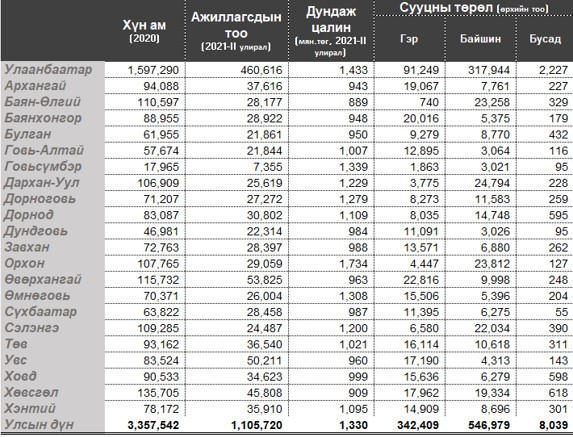
\includegraphics[scale = 0.75]{figures/project1.jpg}  
        % \caption{Statistics of Mongolia}
    \end{table}
\end{frame}

\begin{frame}
\Huge{\centerline{Thank you!}}
\end{frame}

%----------------------------------------------------------------------------------------

\end{document} 